\chapter{Parcours des ressources fournies}
    \section{L'environnement \texttt{Snakemake}}

        \texttt{Snakemake} est un framework permettant de modifier des échelles de données et de créer des fichiers par pipeline. Similaire à \texttt{GNU-Make}, cet outil conçu pour la bio-informatique est utilisé ici pour créer et compresser le dataset de Chicago.

        Le fichier de configuration, appelé \texttt{Snakefile}, comprend une vingtaine d'étapes allant du téléchargement des données jusqu'à la sortie des ensembles  $\mathbb S_{Synth_i}$ par $\mathcal G$. À cet égard il est crucial de comprendre finement son fonctionnement, car il doit être manipulé si l'on veut créer des \textit{Shadow Models} \textit{(voir \ref{SM})}.

        Une fois que la commande \texttt{Snakemake} est terminée, l'équipe peut commencer à travailler avec un dossier comprenant notamment :
        \begin{itemize}
            \item Le dossier \texttt{data} comprenant les datasets $\mathbb{S}_{Pub}$ et $\mathbb{S}_{Synth}$. Les formats utilisés \textit{(\texttt{.parquet, .npz, .pckl})} sont facilement convertissables en dataframes par \texttt{pandas}.
            \item Les scripts nécessaires au fonctionnement de $\mathcal G$
            \item Un certain nombre de fichiers de config \texttt{.yaml}
        \end{itemize}

        Pour des raisons évidentes, les datasets $\mathbb{S}_{Pri}$ sont hachés.

        \begin{tcolorbox}[colback=linkborder_Color!5!white,colframe=linkborder_Color!75!black]
            Le concours étant encore en version \textit{beta}, l'équipe a rencontré de nombreux problèmes lors de l'installation des données fournies. Il est donc préférable à ce stade de développement d'utiliser un environnement Linux et de ne télécharger le dataset initial qu'une fois pour toute l'équipe.
        \end{tcolorbox}

    \newpage\section{Les datasets publics}
        Comme expliqué précédemment, le dataset prend la forme de 7-tuplets de valeurs entre 0
        et 1. On peut alors répartir les valeurs par intervalles pour chaque classe du tuple et
        évaluer leur quantité sur chacun de ces intervalles. Cette représentation visuelle
        élémentaire sera notée $\mathfrak H\left(\mathbb S\right)$ et est donnée ci-dessous.
        \begin{figure}[H]
            \centering
            \subfloat[$\mathfrak H\left( \mathbb{S}_{Pub_{T_{1-2}}}\right)$]{\fbox{
                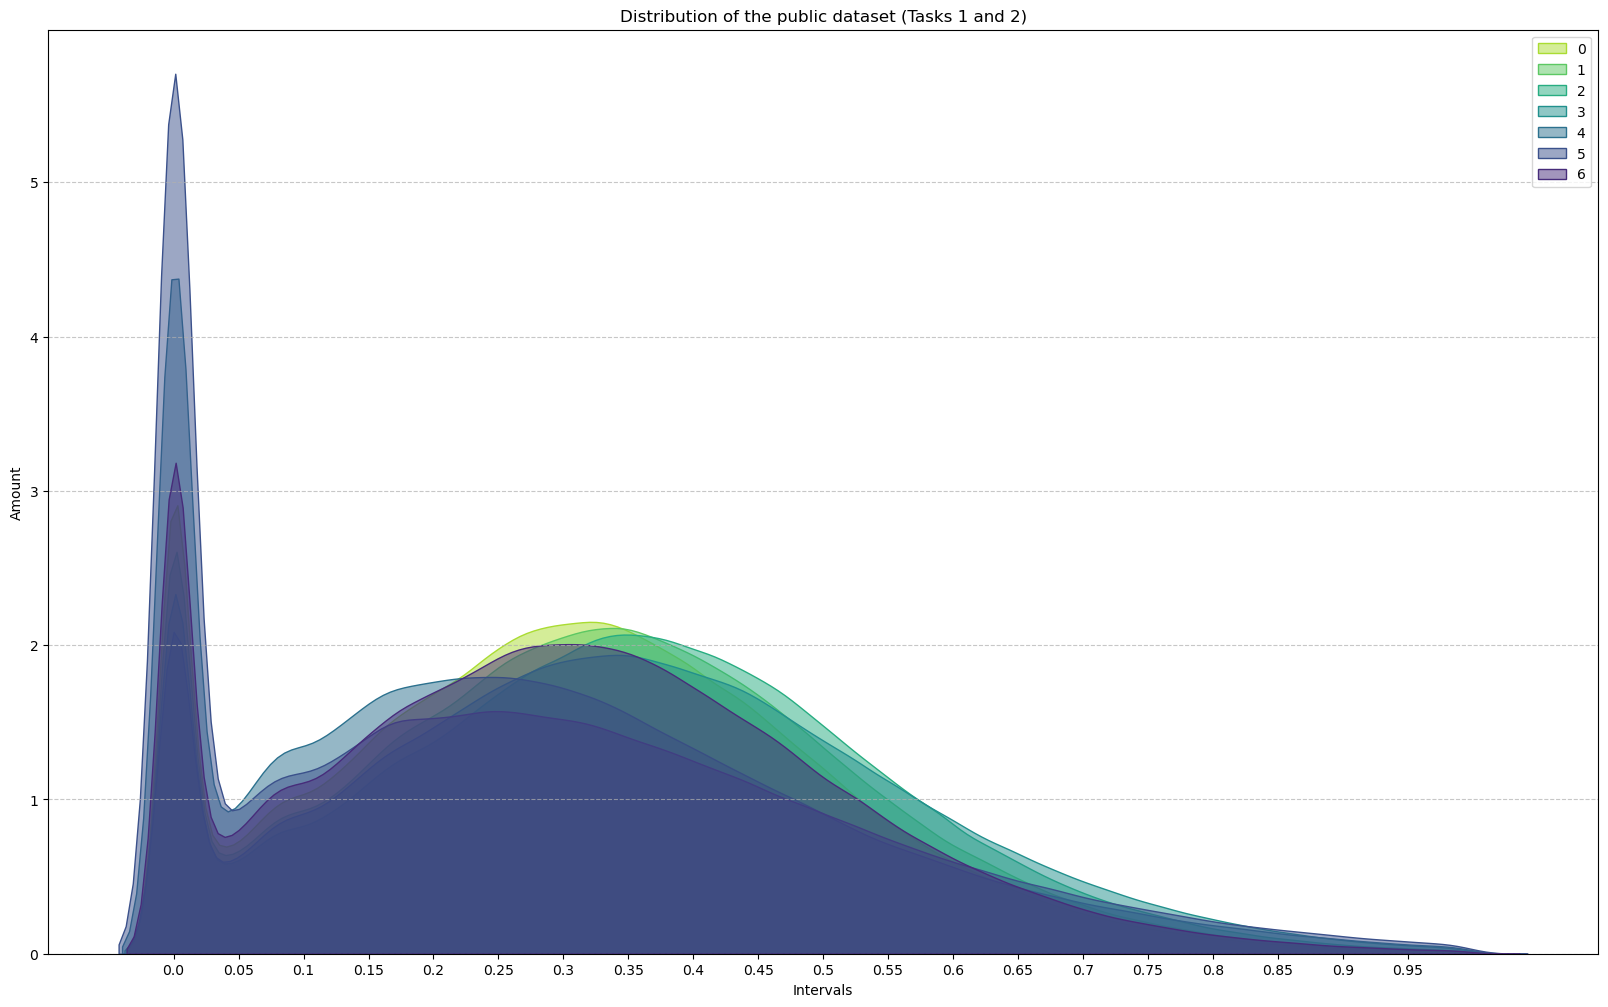
\includegraphics[width = 0.9\textwidth]{figures/Resultats/PublicDS/1&2) PublicDS_ByDays}}}\qquad
            \subfloat[$\mathfrak H\left( \mathbb{S}_{Pub_{T_{3-4}}}\right)$]{\fbox{
                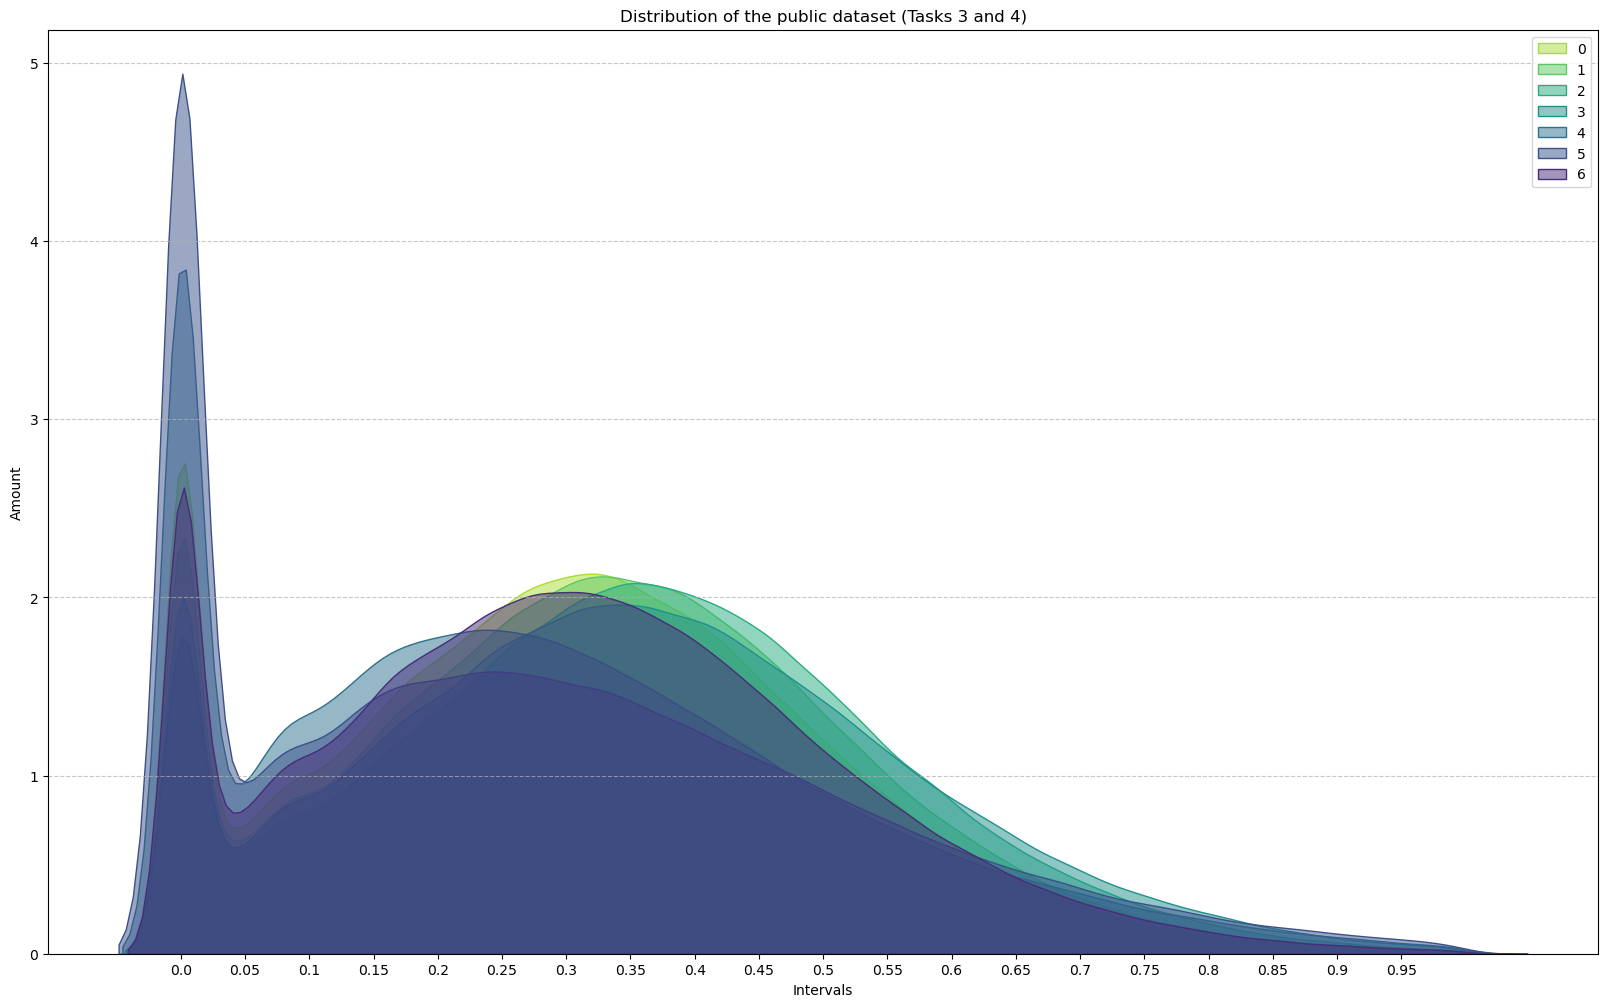
\includegraphics[width = 0.9\textwidth]{figures/Resultats/PublicDS/3&4) PublicDS_ByDays}}}
            \caption{Distribution des données des datasets $\mathbb{S}_{Pub_{T_{1-2}}}$ et
                $\mathbb{S}_{Pub_{T_{3-4}}}$, par jour.}
        \end{figure}


    \section{Les datasets synthétiques}
        \begin{figure}[H]
            \centering
            \subfloat[$\mathfrak H\left( \mathbb{S}_{Priv_{T_{1}}}\right)$]{\fbox{
                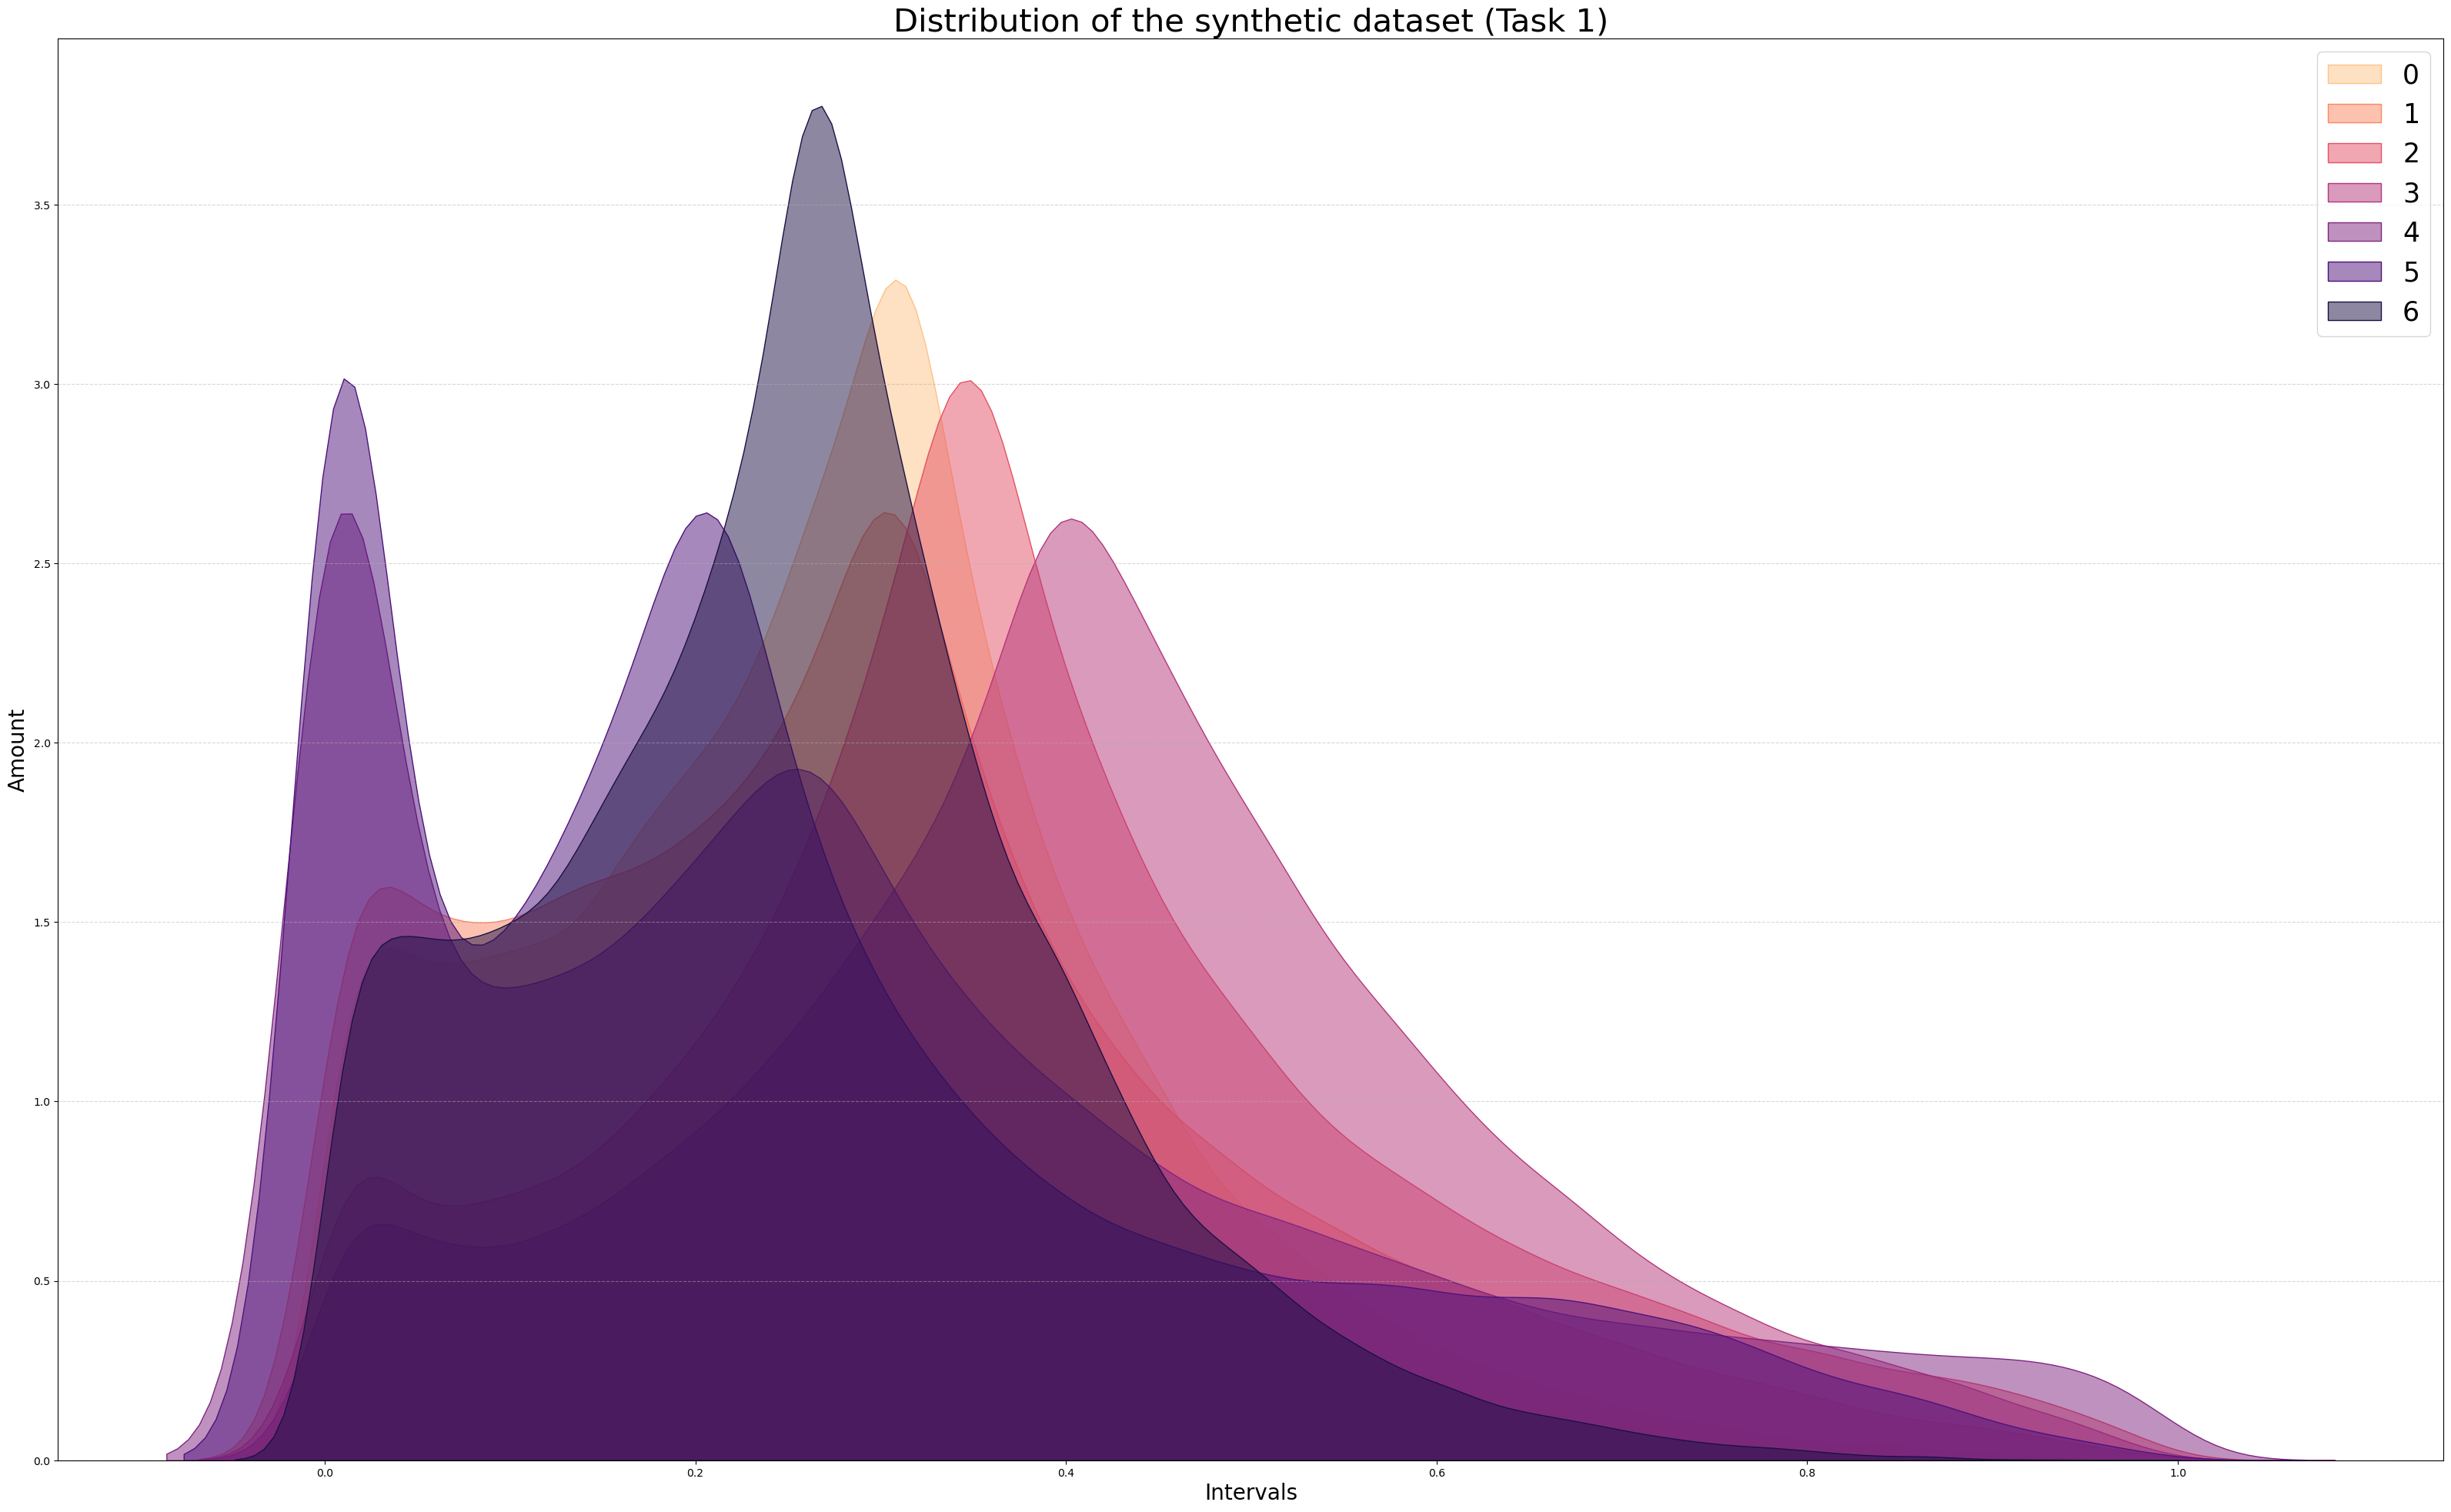
\includegraphics[width = 0.45\textwidth]{figures/Resultats/SyntheticDS/1) SyntheticDS_ByDays}}}\qquad
            ~ %espace entre deux images sur une même ligne
            \subfloat[$\mathfrak H\left( \mathbb{S}_{Priv_{T_{2}}}\right)$]{\fbox{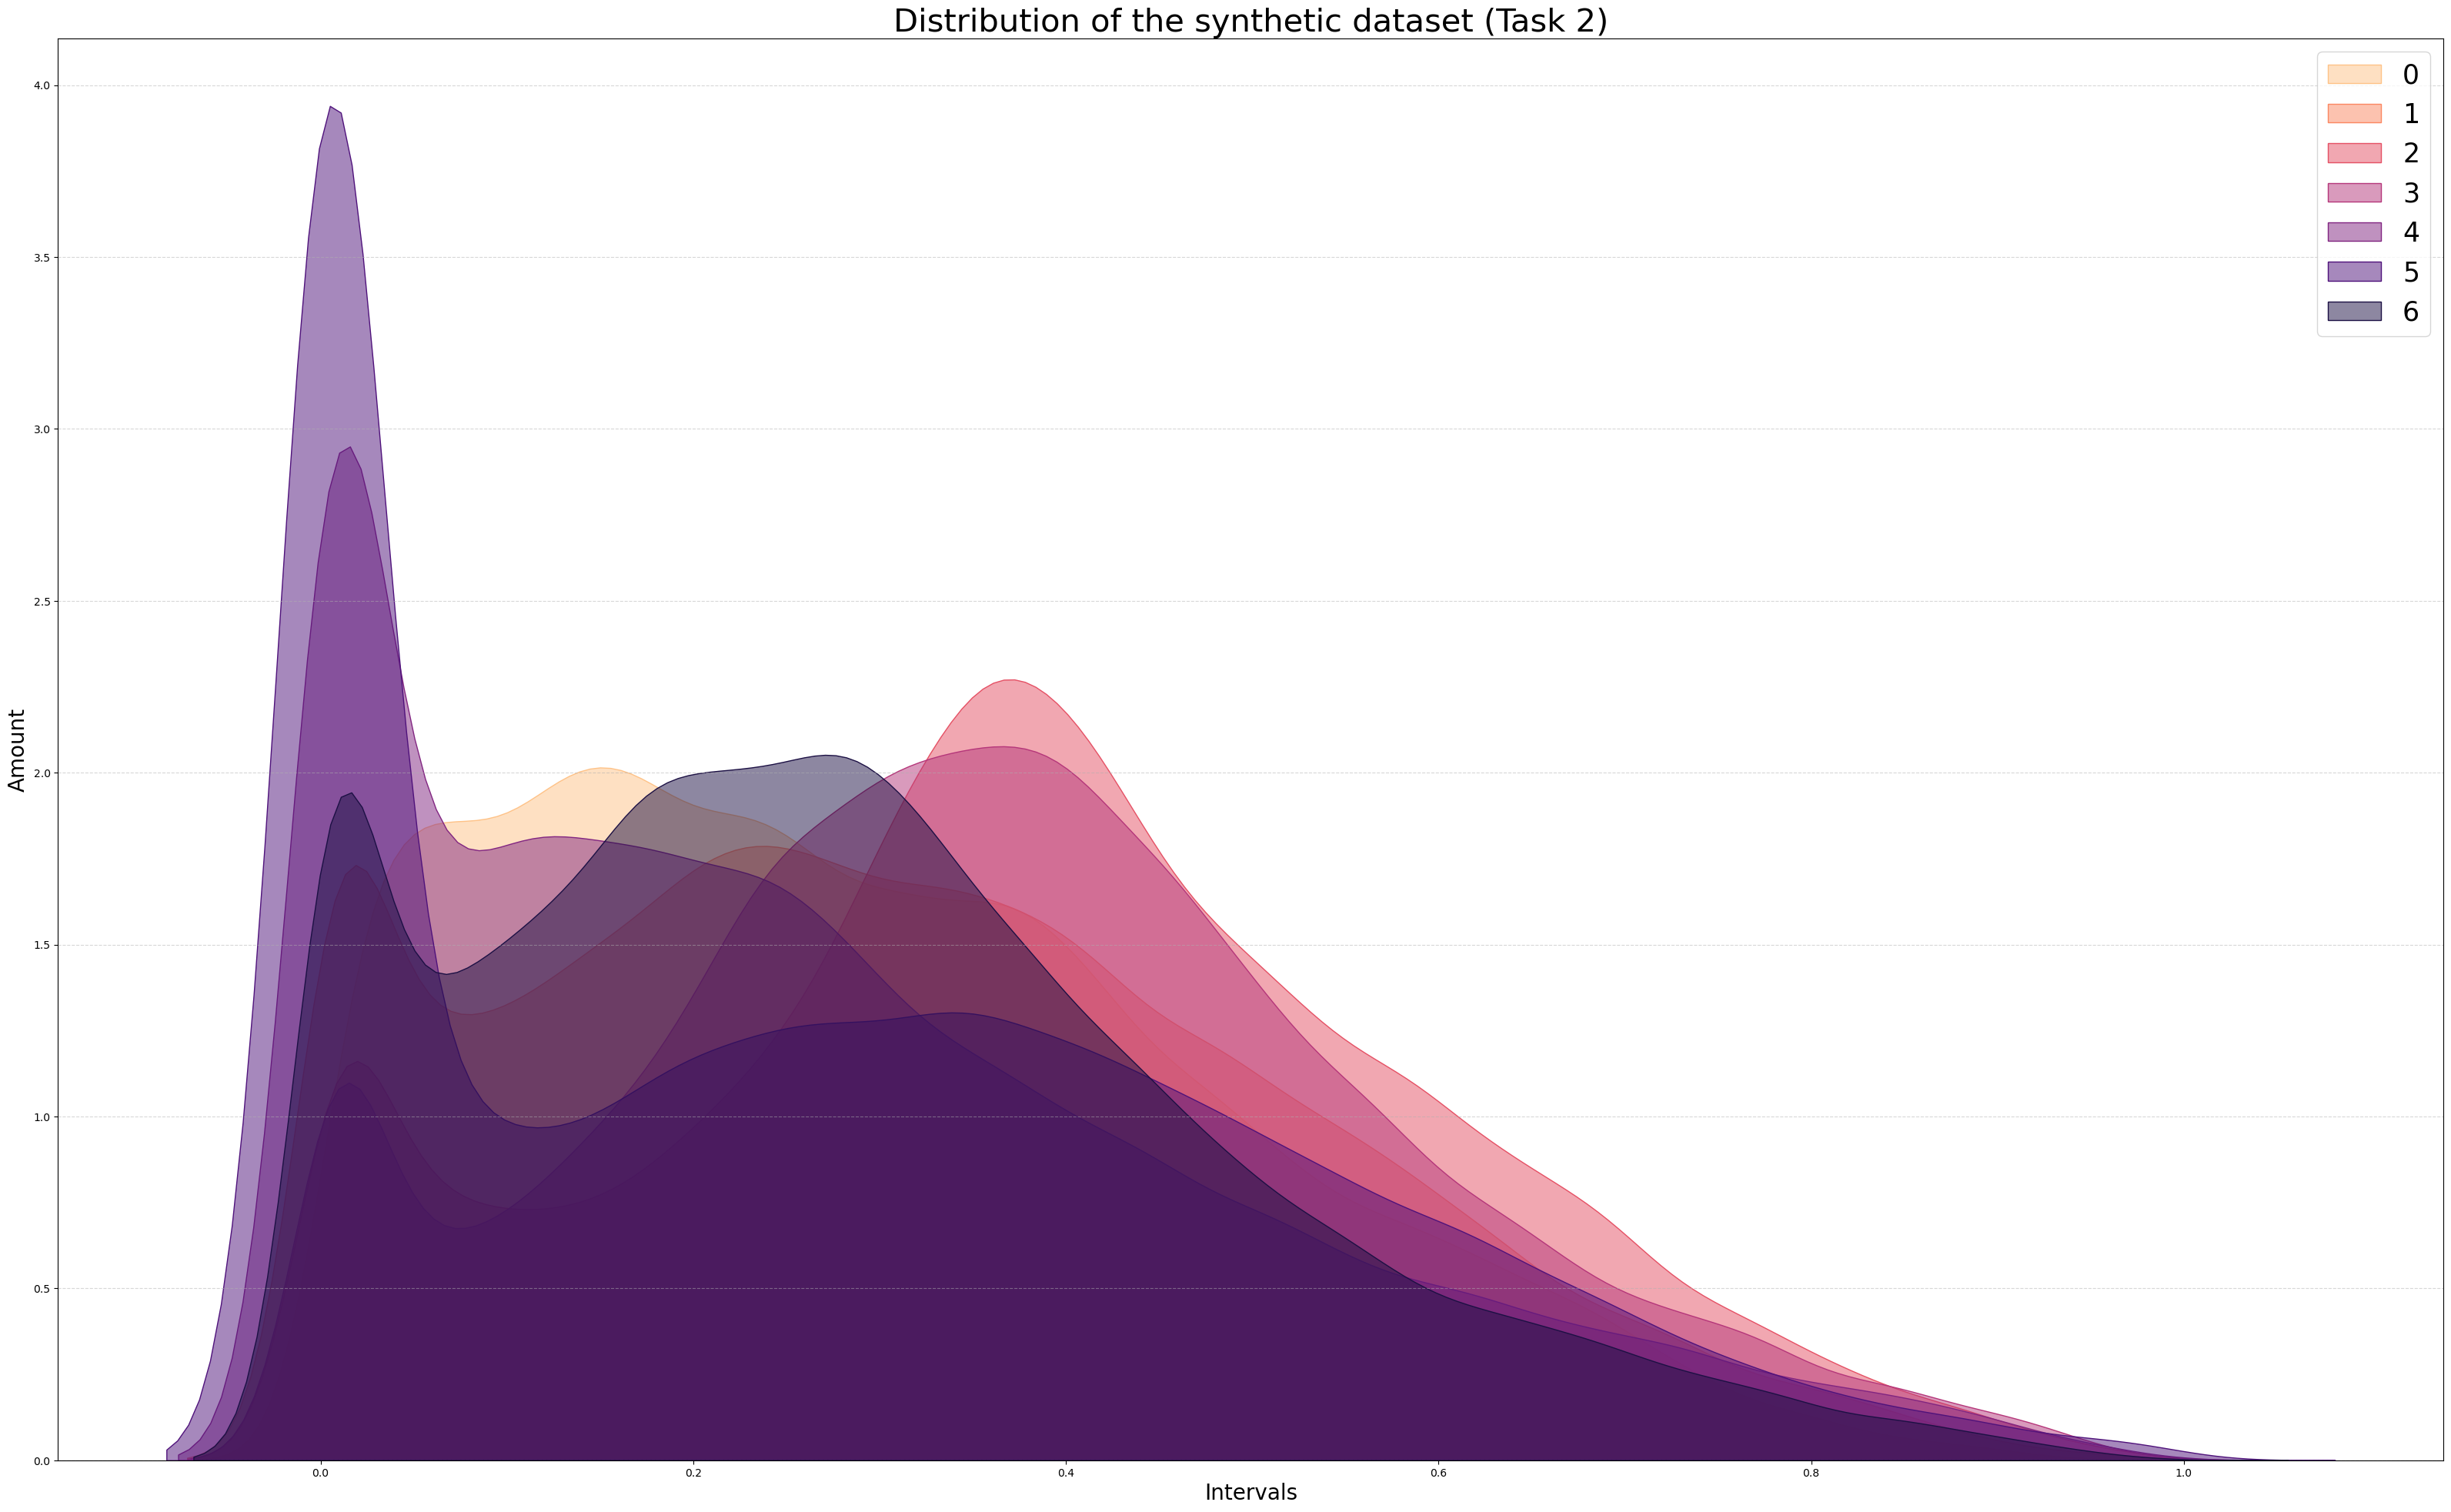
\includegraphics[width = 0.45\textwidth]{figures/Resultats/SyntheticDS/2) SyntheticDS_ByDays}}}\qquad
            \subfloat[$\mathfrak H\left( \mathbb{S}_{Priv_{T_{3}}}\right)$]{\fbox{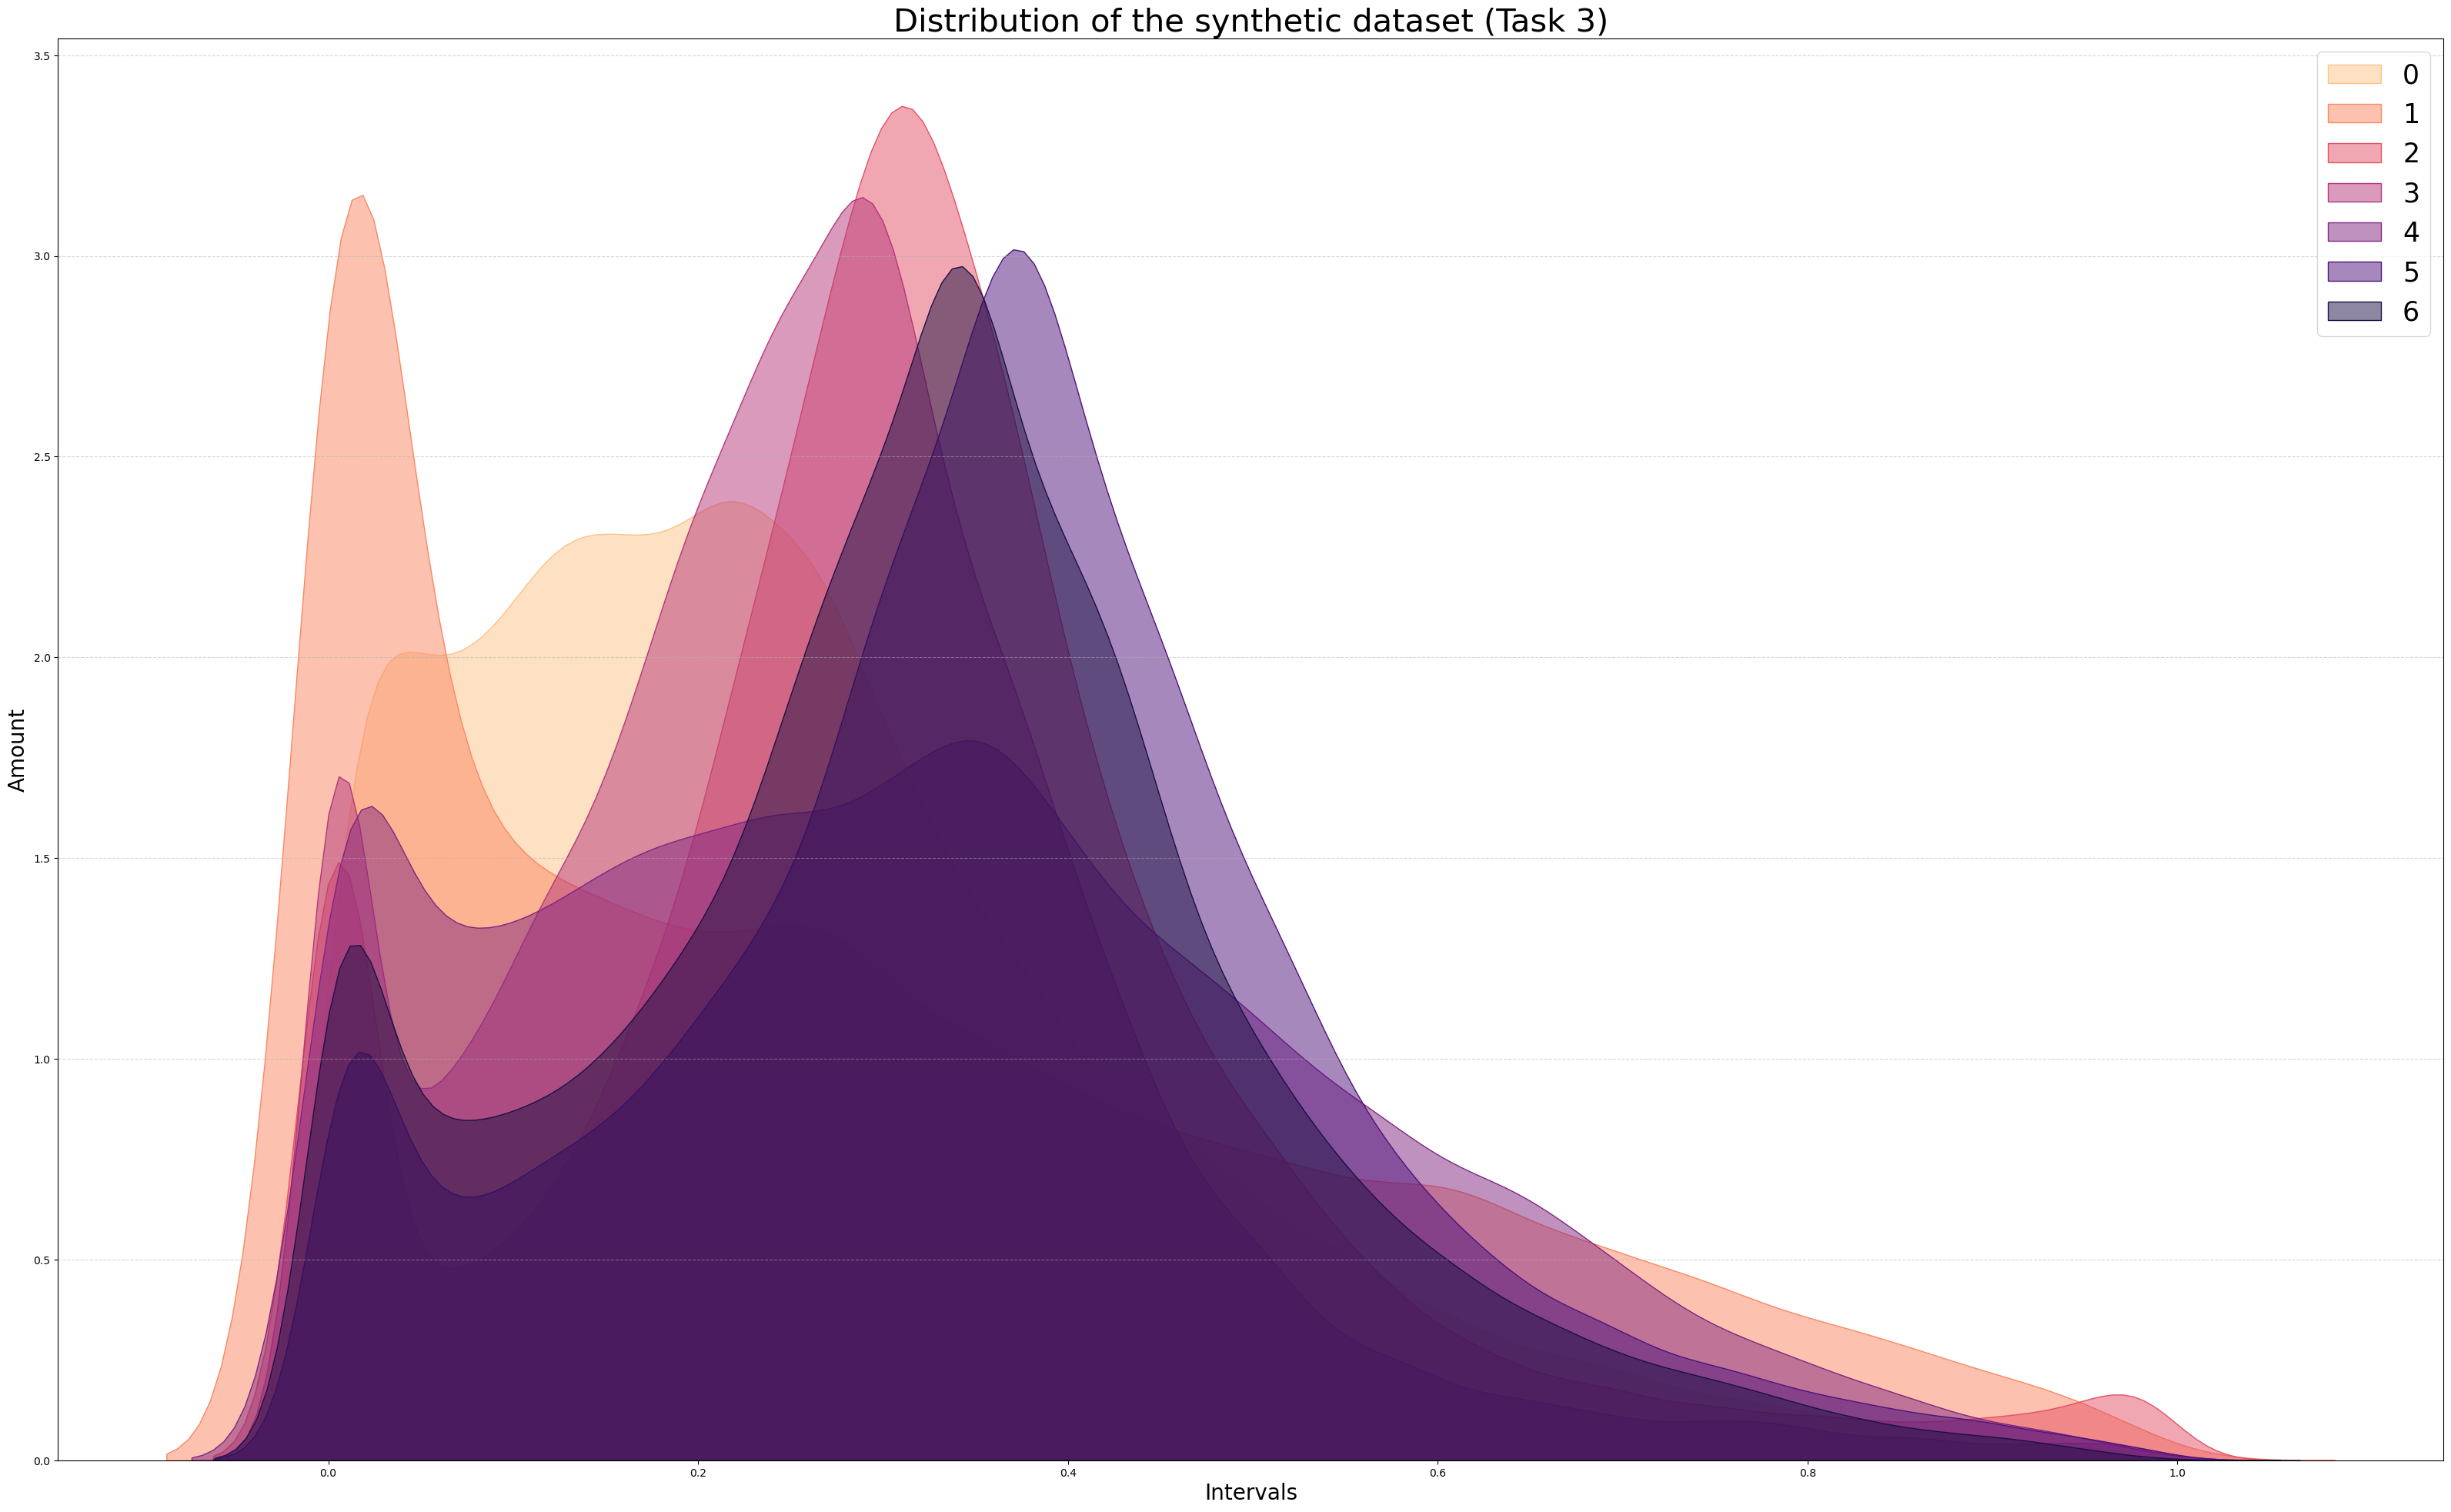
\includegraphics[width = 0.45\textwidth]{figures/Resultats/SyntheticDS/3) SyntheticDS_ByDays}}}\qquad
            ~ %espace entre deux images sur une même ligne
            \subfloat[$\mathfrak H\left( \mathbb{S}_{Priv_{T_{4}}}\right)$]{\fbox{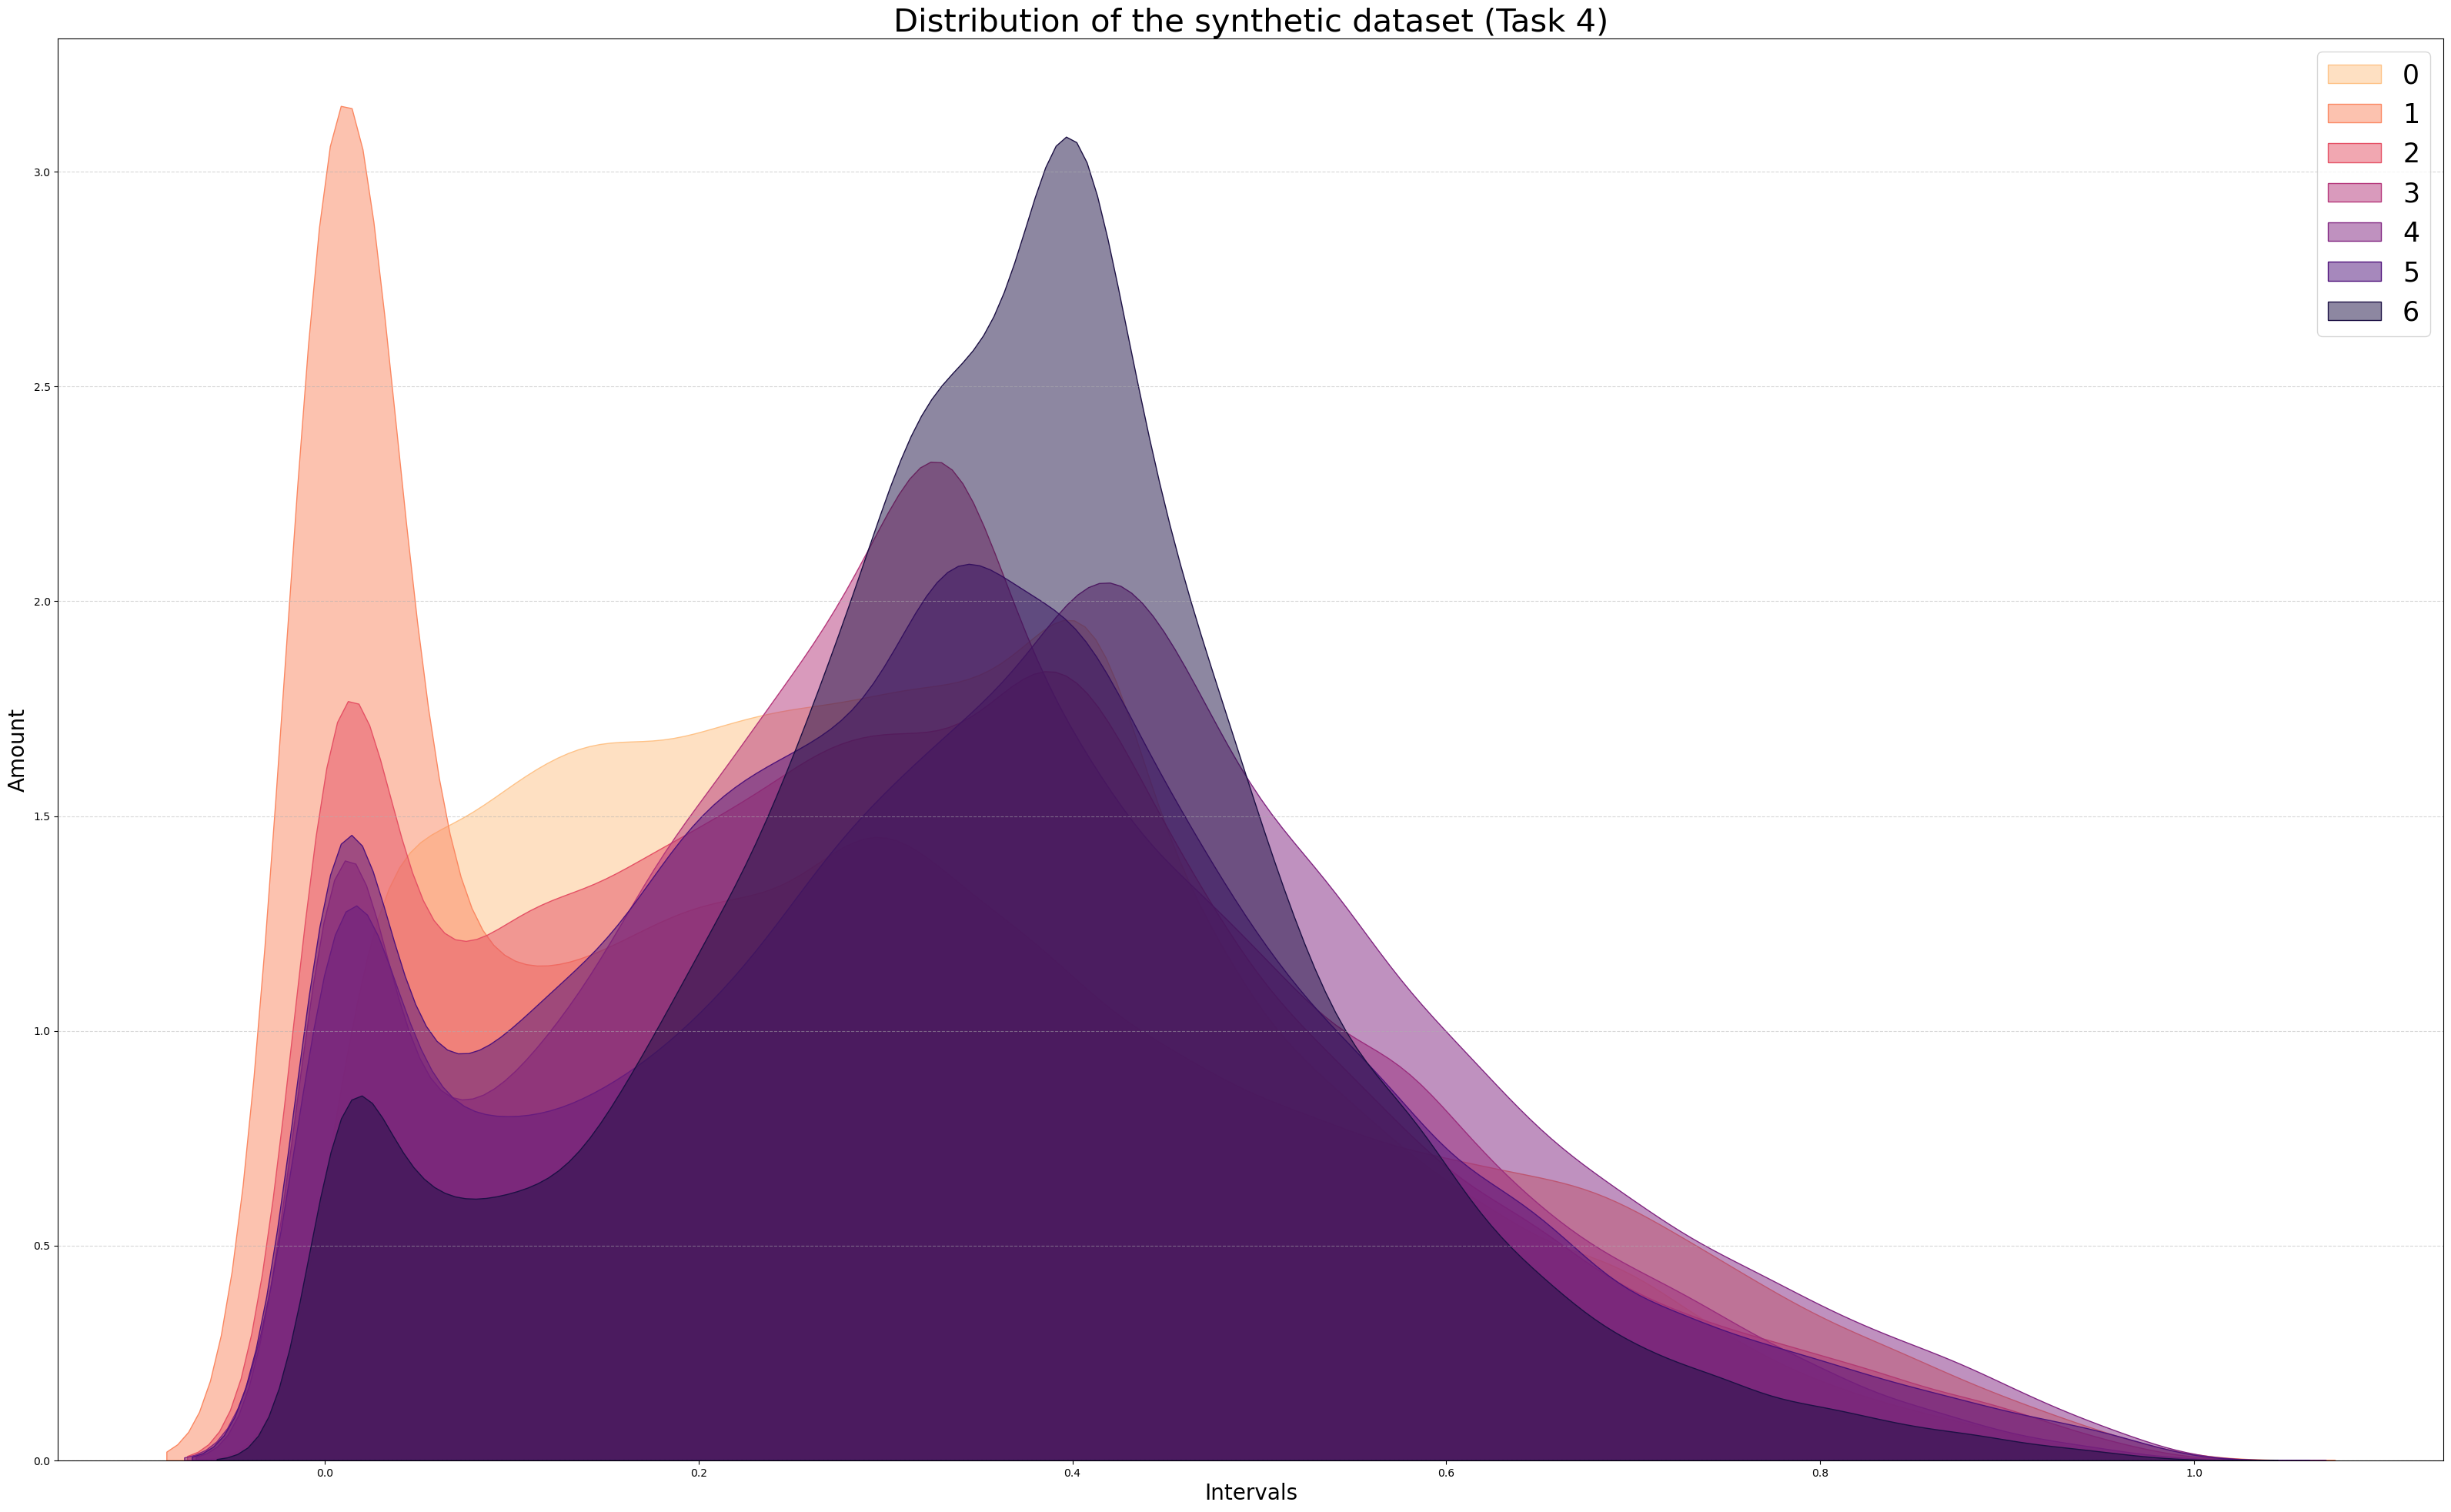
\includegraphics[width = 0.45\textwidth]{figures/Resultats/SyntheticDS/4) SyntheticDS_ByDays}}}
            \caption{Distribution des données des datasets $\mathbb{S}_{Synth_i}$, par jour.}
        \end{figure}